% Topic T1.1: What Is Money, Really?
% Self-contained Beamer slides for Digital Finance course
\documentclass[11pt,aspectratio=169]{beamer}
\usetheme{Madrid}

% ======================= PACKAGES =======================
\usepackage{graphicx}
\usepackage{booktabs}
\usepackage{adjustbox}
\usepackage{multicol}
\usepackage{amsmath}
\usepackage{amssymb}
\usepackage{tikz}
\usetikzlibrary{arrows,shapes,positioning,shadows,trees}
\usepackage{listings}
\usepackage{xcolor}

% ======================= COLOR DEFINITIONS =======================
% Primary color scheme: Blue/Teal for Digital Finance
\definecolor{dfblue}{RGB}{0,102,204}
\definecolor{dfteal}{RGB}{0,153,153}
\definecolor{dfcyan}{RGB}{51,187,204}
\definecolor{dflightblue}{RGB}{153,204,255}
\definecolor{dflightblue2}{RGB}{173,214,255}
\definecolor{dflightblue3}{RGB}{193,224,255}
\definecolor{dflightblue4}{RGB}{213,234,255}

% Accent colors for finance applications
\definecolor{dfgreen}{RGB}{44, 160, 44}
\definecolor{dfred}{RGB}{214, 39, 40}
\definecolor{dforange}{RGB}{255, 127, 14}
\definecolor{dfgray}{RGB}{127, 127, 127}

% Utility colors
\definecolor{lightgray}{RGB}{240, 240, 240}
\definecolor{midgray}{RGB}{180, 180, 180}
\definecolor{codebg}{RGB}{245, 245, 245}

% ======================= THEME CUSTOMIZATION =======================
% Apply Digital Finance color scheme to Madrid theme
\setbeamercolor{palette primary}{bg=dflightblue3,fg=dfblue}
\setbeamercolor{palette secondary}{bg=dflightblue2,fg=dfblue}
\setbeamercolor{palette tertiary}{bg=dfteal,fg=white}
\setbeamercolor{palette quaternary}{bg=dfblue,fg=white}

\setbeamercolor{structure}{fg=dfblue}
\setbeamercolor{section in toc}{fg=dfblue}
\setbeamercolor{subsection in toc}{fg=dfteal}
\setbeamercolor{title}{fg=dfblue}
\setbeamercolor{frametitle}{fg=dfblue,bg=dflightblue3}
\setbeamercolor{block title}{bg=dflightblue2,fg=dfblue}
\setbeamercolor{block body}{bg=dflightblue4,fg=black}

% Remove navigation symbols for cleaner look
\setbeamertemplate{navigation symbols}{}

% Clean itemize/enumerate
\setbeamertemplate{itemize items}[circle]
\setbeamertemplate{enumerate items}[default]

% Margins for readability
\setbeamersize{text margin left=8mm,text margin right=8mm}

% ======================= LISTINGS CONFIGURATION =======================
% Python code style
\lstdefinestyle{pythonstyle}{
    language=Python,
    basicstyle=\ttfamily\footnotesize,
    keywordstyle=\color{dfblue}\bfseries,
    stringstyle=\color{dforange},
    commentstyle=\color{dfgray}\itshape,
    numberstyle=\tiny\color{dfgray},
    numbers=left,
    numbersep=5pt,
    backgroundcolor=\color{codebg},
    showspaces=false,
    showstringspaces=false,
    showtabs=false,
    frame=single,
    rulecolor=\color{midgray},
    tabsize=4,
    captionpos=b,
    breaklines=true,
    breakatwhitespace=false,
    escapeinside={(*@}{@*)},
    xleftmargin=10pt,
    xrightmargin=10pt
}

% Solidity code style
\lstdefinestyle{soliditystyle}{
    language=Java, % closest approximation
    basicstyle=\ttfamily\footnotesize,
    keywordstyle=\color{dfteal}\bfseries,
    stringstyle=\color{dforange},
    commentstyle=\color{dfgray}\itshape,
    numberstyle=\tiny\color{dfgray},
    numbers=left,
    numbersep=5pt,
    backgroundcolor=\color{codebg},
    showspaces=false,
    showstringspaces=false,
    showtabs=false,
    frame=single,
    rulecolor=\color{midgray},
    tabsize=2,
    captionpos=b,
    breaklines=true,
    breakatwhitespace=false,
    escapeinside={(*@}{@*)},
    xleftmargin=10pt,
    xrightmargin=10pt,
    morekeywords={pragma, contract, function, returns, public, private, view, pure, payable, address, uint256, mapping, event, modifier}
}

% Inline code command
\newcommand{\code}[1]{\texttt{\color{dfblue}#1}}

% ======================= CUSTOM COMMANDS =======================
% Bottom annotation (Madrid-style)
\newcommand{\bottomnote}[1]{%
\vfill
\vspace{-2mm}
\textcolor{dflightblue2}{\rule{\textwidth}{0.4pt}}
\vspace{1mm}
\footnotesize
\textbf{#1}
}

% Compact list spacing
\newcommand{\compactlist}{%
\setlength{\itemsep}{0pt}%
\setlength{\parskip}{0pt}%
\setlength{\parsep}{0pt}%
}

% Chart placeholder
\newcommand{\chartplaceholder}[2][5cm]{%
\begin{center}
\begin{adjustbox}{max width=0.95\textwidth, max height=#1}
\framebox[\textwidth][c]{%
\rule{0pt}{#1}%
\textcolor{midgray}{[#2]}%
}
\end{adjustbox}
\end{center}
}

% ======================= FINANCE NOTATION MACROS =======================
% Probability and statistics
\newcommand{\E}{\mathbb{E}} % Expected value
\newcommand{\Var}{\mathrm{Var}} % Variance
\newcommand{\Cov}{\mathrm{Cov}} % Covariance
\newcommand{\Prob}{\mathbb{P}} % Probability

% Distributions
\newcommand{\Normal}{\mathcal{N}} % Normal distribution
\newcommand{\Uniform}{\mathcal{U}} % Uniform distribution

% Returns and prices
\newcommand{\Ret}{R} % Return
\newcommand{\LogRet}{r} % Log return
\newcommand{\Price}{S} % Price/Stock price
\newcommand{\Strike}{K} % Strike price

% Options and derivatives
\newcommand{\CallPrice}{C} % Call option price
\newcommand{\PutPrice}{P} % Put option price
\newcommand{\Greeks}[1]{\mathit{#1}} % Greek letters

% Risk measures
\newcommand{\VaR}{\mathrm{VaR}} % Value at Risk
\newcommand{\CVaR}{\mathrm{CVaR}} % Conditional VaR
\newcommand{\Sharpe}{\mathrm{SR}} % Sharpe Ratio

% Time series
\newcommand{\AR}{\mathrm{AR}} % Autoregressive
\newcommand{\MA}{\mathrm{MA}} % Moving average
\newcommand{\GARCH}{\mathrm{GARCH}} % GARCH

% Blockchain/Crypto
\newcommand{\Hash}{\mathrm{Hash}} % Hash function
\newcommand{\Block}{\mathcal{B}} % Block
\newcommand{\Chain}{\mathcal{C}} % Chain

% Real numbers, integers
\newcommand{\R}{\mathbb{R}}
\newcommand{\Z}{\mathbb{Z}}
\newcommand{\N}{\mathbb{N}}

% ======================= TIKZ STYLES =======================
% Styles for finance-related diagrams
\tikzstyle{process} = [rectangle, minimum width=3cm, minimum height=1cm, text centered, draw=dfblue, fill=dflightblue4, thick]
\tikzstyle{decision} = [diamond, minimum width=3cm, minimum height=1cm, text centered, draw=dfteal, fill=dflightblue4, thick]
\tikzstyle{arrow} = [thick,->,>=stealth,color=dfblue]
\tikzstyle{blockchain} = [rectangle, rounded corners, minimum width=2.5cm, minimum height=1cm, text centered, draw=dfteal, fill=dflightblue3, thick]
\tikzstyle{transaction} = [circle, minimum size=0.8cm, text centered, draw=dforange, fill=dflightblue4, thick]

% ======================= FOOTER TEMPLATE =======================
\setbeamertemplate{footline}{
    \hbox{\begin{beamercolorbox}[wd=\paperwidth,ht=2.5ex,dp=1ex,leftskip=.5em,rightskip=.5em]{author in head/foot}
    \tiny
    \textbf{Digital Finance} \hfill
    Joerg Osterrieder \hfill
    \insertdate \hfill
    Page \insertframenumber{} / \inserttotalframenumber
    \end{beamercolorbox}}
}

% ======================= SECTION DIVIDER TEMPLATE =======================
\AtBeginSection[]{
\begin{frame}[plain]
\vfill
\centering
\begin{beamercolorbox}[sep=12pt,center]{title}
\usebeamerfont{title}\LARGE\insertsection\par
\end{beamercolorbox}
\vfill
\end{frame}
}


\title[T1.1: What Is Money?]{Topic 1.1: What Is Money, Really?}
\subtitle{Trust, Ledgers, and the Double-Spending Problem}
\author{Joerg Osterrieder}
\institute{Digital Finance}
\date{2025}

\begin{document}

% =============================================================================
% Frame 1: Title Slide
% =============================================================================
\begin{frame}[plain]
\titlepage
\end{frame}

% =============================================================================
% Frame 2: Learning Objectives
% =============================================================================
\begin{frame}{Learning Objectives}
\begin{center}
\textbf{\Large What You Will Learn in This Topic}
\end{center}

\vspace{5mm}
By the end of this session, you will be able to:

\begin{enumerate}
\item \textbf{Dissolve assumptions} about what money ``is''
\item \textbf{Understand} why digital money is fundamentally hard
\item \textbf{Explain} the double-spending problem and its implications
\item \textbf{Distinguish} account-based from token-based money
\item \textbf{Analyze} the trade-offs of trusted intermediaries
\end{enumerate}

\vspace{5mm}
\begin{block}{Hands-On Component}
We'll use a Colab notebook to simulate a simple ledger and see double-spending in action.
\end{block}
\end{frame}

% =============================================================================
% Frame 3: Prerequisites/Background I
% =============================================================================
\begin{frame}{Prerequisites: What You Should Know}
\begin{columns}[T]
\begin{column}{0.48\textwidth}
\textbf{No prior knowledge required!}
\begin{itemize}
\item This topic starts from first principles
\item We'll build up concepts step by step
\item Questions are encouraged
\end{itemize}

\vspace{3mm}
\textbf{Helpful background:}
\begin{itemize}
\item Basic understanding of banks
\item Familiarity with digital payments
\item Curiosity about how things work
\end{itemize}
\end{column}
\begin{column}{0.48\textwidth}
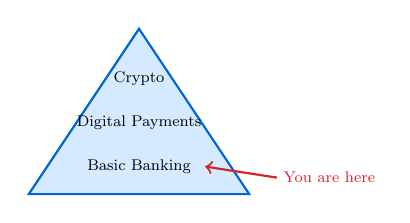
\begin{tikzpicture}[scale=0.7, transform shape]
% Knowledge pyramid
\draw[thick, dfblue, fill=dflightblue4] (0,0) -- (4,0) -- (2,3) -- cycle;
\node at (2,0.5) {\footnotesize Basic Banking};
\node at (2,1.3) {\footnotesize Digital Payments};
\node at (2,2.1) {\footnotesize Crypto};
\draw[dfred, thick, ->] (4.5,0.3) -- (3.2,0.5);
\node[right] at (4.5,0.3) {\footnotesize \textcolor{dfred}{You are here}};
\end{tikzpicture}
\end{column}
\end{columns}

\vspace{3mm}
\begin{alertblock}{Key Mindset}
Forget everything you ``know'' about money. We're going to rebuild the concept from scratch.
\end{alertblock}
\end{frame}

% =============================================================================
% Frame 4: Prerequisites/Background II
% =============================================================================
\begin{frame}{The Big Picture: Why This Matters}
\begin{center}
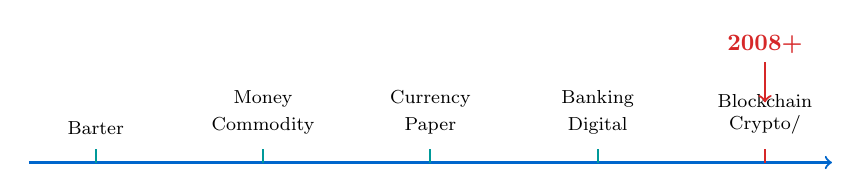
\begin{tikzpicture}[scale=0.85, transform shape]
% Timeline
\draw[thick, dfblue, ->] (0,0) -- (12,0);

% Milestones
\node[above] at (1,0.3) {\footnotesize Barter};
\draw[thick, dfteal] (1,0) -- (1,0.2);

\node[above] at (3.5,0.3) {\footnotesize Commodity};
\node[above] at (3.5,0.7) {\footnotesize Money};
\draw[thick, dfteal] (3.5,0) -- (3.5,0.2);

\node[above] at (6,0.3) {\footnotesize Paper};
\node[above] at (6,0.7) {\footnotesize Currency};
\draw[thick, dfteal] (6,0) -- (6,0.2);

\node[above] at (8.5,0.3) {\footnotesize Digital};
\node[above] at (8.5,0.7) {\footnotesize Banking};
\draw[thick, dfteal] (8.5,0) -- (8.5,0.2);

\node[above] at (11,0.3) {\footnotesize Crypto/};
\node[above] at (11,0.7) {\footnotesize Blockchain};
\draw[thick, dfred] (11,0) -- (11,0.2);

% You are here
\draw[dfred, thick, ->] (11,1.5) -- (11,0.9);
\node[above] at (11,1.5) {\textcolor{dfred}{\textbf{2008+}}};
\end{tikzpicture}
\end{center}

\vspace{3mm}
\textbf{We're witnessing a fundamental shift:}
\begin{itemize}
\item Money is being \textbf{reinvented} for the digital age
\item Old assumptions are being \textbf{challenged}
\item New possibilities are \textbf{emerging}
\end{itemize}

\vspace{3mm}
\begin{block}{Course Goal}
Understand \textit{why} these changes are happening and \textit{how} they work.
\end{block}
\end{frame}

% =============================================================================
% Frame 5: A Thought Experiment
% =============================================================================
\begin{frame}{A Thought Experiment}
\begin{center}
\textbf{\Large Imagine you're stranded on an island with 9 strangers...}
\end{center}

\vspace{5mm}
\begin{columns}[T]
\begin{column}{0.5\textwidth}
\textbf{You have skills:}
\begin{itemize}
\item Alice: fishing
\item Bob: building
\item Carol: farming
\item Dave: medicine
\item ...and so on
\end{itemize}
\end{column}
\begin{column}{0.5\textwidth}
\textbf{The problem:}
\begin{itemize}
\item Alice wants vegetables
\item Carol doesn't need fish
\item How do you trade?
\end{itemize}
\end{column}
\end{columns}

\vspace{5mm}
\begin{alertblock}{The Coincidence of Wants Problem}
Direct barter requires both parties to want what the other has, at the same time. This almost never happens.
\end{alertblock}
\end{frame}

% =============================================================================
% Frame 6: Three Solutions to the Barter Problem
% =============================================================================
\begin{frame}{Three Solutions to the Barter Problem}
\begin{center}
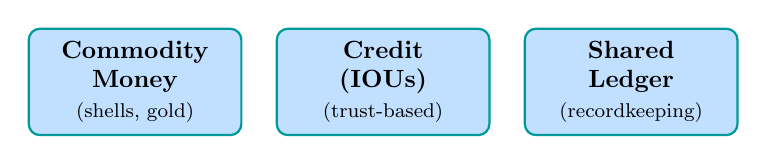
\begin{tikzpicture}[node distance=3.5cm, scale=0.9, transform shape]
% Solution 1: Commodity Money
\node (commodity) [blockchain, minimum width=3cm, minimum height=1.5cm] {
\begin{tabular}{c}
\textbf{Commodity}\\
\textbf{Money}\\
\footnotesize (shells, gold)
\end{tabular}
};

% Solution 2: Credit/Debt
\node (credit) [blockchain, right of=commodity, minimum width=3cm, minimum height=1.5cm] {
\begin{tabular}{c}
\textbf{Credit}\\
\textbf{(IOUs)}\\
\footnotesize (trust-based)
\end{tabular}
};

% Solution 3: Ledger
\node (ledger) [blockchain, right of=credit, minimum width=3cm, minimum height=1.5cm] {
\begin{tabular}{c}
\textbf{Shared}\\
\textbf{Ledger}\\
\footnotesize (recordkeeping)
\end{tabular}
};

\end{tikzpicture}
\end{center}

\vspace{5mm}
\textbf{Key Insight:} All three solutions are really about \textcolor{dfblue}{\textbf{trust}}.
\begin{itemize}
\item Commodity: Trust the material has value
\item Credit: Trust the person will repay
\item Ledger: Trust the recordkeeper is honest
\end{itemize}
\end{frame}

% =============================================================================
% Frame 7: Money as a Social Technology
% =============================================================================
\begin{frame}{Money as a Social Technology}
\begin{columns}[T]
\begin{column}{0.55\textwidth}
\textbf{Think about the last time you paid for something...}

\vspace{2mm}
\textbf{The Three Functions of Money:}
\begin{enumerate}
\item \textbf{Medium of Exchange}\\
\footnotesize Accepted for transactions\\
\footnotesize \textcolor{dfteal}{Example: Your Starbucks gift card is a medium of exchange---but only within Starbucks}
\item \textbf{Unit of Account}\\
\footnotesize Common measure of value
\item \textbf{Store of Value}\\
\footnotesize Holds purchasing power over time
\end{enumerate}

\vspace{2mm}
\textbf{What makes something ``money''?}\\
\textcolor{dfteal}{Collective belief that others will accept it.}
\end{column}
\begin{column}{0.42\textwidth}
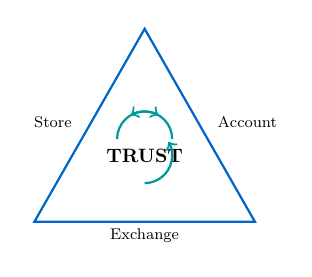
\begin{tikzpicture}[scale=0.7, transform shape]
% Triangle of money functions
\coordinate (A) at (0,0);
\coordinate (B) at (4,0);
\coordinate (C) at (2,3.5);

\draw[thick, dfblue] (A) -- (B) -- (C) -- cycle;

\node at (2,1.2) {\textbf{TRUST}};
\node[below] at (2,0) {\footnotesize Exchange};
\node[left] at (0.8,1.8) {\footnotesize Store};
\node[right] at (3.2,1.8) {\footnotesize Account};

% Add circular arrows suggesting interconnection
\draw[->, dfteal, thick] (1.5,1.5) arc (180:60:0.5);
\draw[->, dfteal, thick] (2.5,1.5) arc (0:120:0.5);
\draw[->, dfteal, thick] (2,0.7) arc (-90:30:0.5);
\end{tikzpicture}
\end{column}
\end{columns}

\vspace{3mm}
\begin{block}{Anthropological Fact}
Debt and credit systems (ledgers) predate physical currency by thousands of years. Money is fundamentally about \textbf{information}, not objects.
\end{block}
\end{frame}

% =============================================================================
% Frame 8: Historical Evolution of Money
% =============================================================================
\begin{frame}{Historical Evolution of Money}
\begin{center}
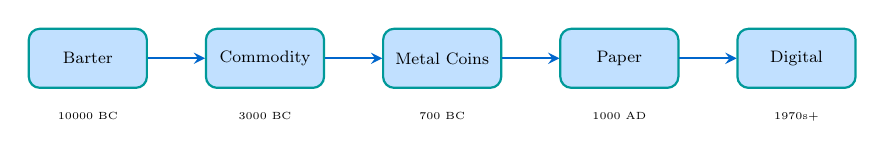
\begin{tikzpicture}[scale=0.75, transform shape]
% Stages
\node[blockchain, minimum width=2cm] (stage1) at (0,0) {\footnotesize Barter};
\node[blockchain, minimum width=2cm] (stage2) at (3,0) {\footnotesize Commodity};
\node[blockchain, minimum width=2cm] (stage3) at (6,0) {\footnotesize Metal Coins};
\node[blockchain, minimum width=2cm] (stage4) at (9,0) {\footnotesize Paper};
\node[blockchain, minimum width=2cm] (stage5) at (12,0) {\footnotesize Digital};

% Arrows
\draw[arrow] (stage1) -- (stage2);
\draw[arrow] (stage2) -- (stage3);
\draw[arrow] (stage3) -- (stage4);
\draw[arrow] (stage4) -- (stage5);

% Labels below
\node[below] at (0,-0.8) {\tiny 10000 BC};
\node[below] at (3,-0.8) {\tiny 3000 BC};
\node[below] at (6,-0.8) {\tiny 700 BC};
\node[below] at (9,-0.8) {\tiny 1000 AD};
\node[below] at (12,-0.8) {\tiny 1970s+};
\end{tikzpicture}
\end{center}

\vspace{3mm}
\begin{columns}[T]
\begin{column}{0.48\textwidth}
\textbf{Key Pattern:}
\begin{itemize}
\item Each stage = more \textbf{abstract}
\item Each stage = more \textbf{scalable}
\item Each stage = requires more \textbf{trust}
\end{itemize}

\vspace{2mm}
\textbf{Why did gold win?}
\begin{itemize}\compactlist
\item Durable (doesn't rot)
\item Divisible (can be split)
\item Portable (easy to carry)
\item Recognizable (hard to fake)
\item Scarce (limited supply)
\end{itemize}
\end{column}
\begin{column}{0.48\textwidth}
\textbf{The Constant:}
\begin{itemize}
\item \textcolor{dfteal}{Always about trust}
\item \textcolor{dfteal}{Always about recordkeeping}
\item \textcolor{dfteal}{Always social technology}
\end{itemize}
\end{column}
\end{columns}
\end{frame}

% =============================================================================
% Frame 9: The Ledger - Humanity's Oldest Financial Technology
% =============================================================================
\begin{frame}{The Ledger: Humanity's Oldest Financial Technology}
\begin{center}
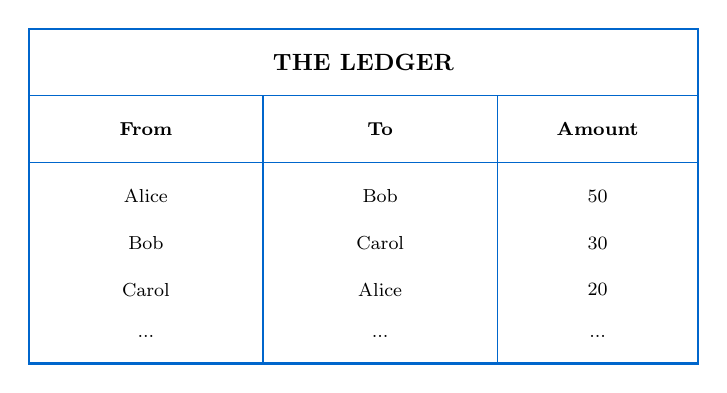
\begin{tikzpicture}[scale=0.85, transform shape]
% Simple ledger representation
\draw[thick, dfblue] (0,0) rectangle (10,5);
\node at (5,4.5) {\textbf{THE LEDGER}};
\draw[dfblue] (0,4) -- (10,4);

% Header
\draw[dfblue] (3.5,4) -- (3.5,0);
\draw[dfblue] (7,4) -- (7,0);
\node at (1.75,3.5) {\footnotesize \textbf{From}};
\node at (5.25,3.5) {\footnotesize \textbf{To}};
\node at (8.5,3.5) {\footnotesize \textbf{Amount}};
\draw[dfblue] (0,3) -- (10,3);

% Transactions
\node at (1.75,2.5) {\footnotesize Alice};
\node at (5.25,2.5) {\footnotesize Bob};
\node at (8.5,2.5) {\footnotesize 50};

\node at (1.75,1.8) {\footnotesize Bob};
\node at (5.25,1.8) {\footnotesize Carol};
\node at (8.5,1.8) {\footnotesize 30};

\node at (1.75,1.1) {\footnotesize Carol};
\node at (5.25,1.1) {\footnotesize Alice};
\node at (8.5,1.1) {\footnotesize 20};

\node at (1.75,0.4) {\footnotesize ...};
\node at (5.25,0.4) {\footnotesize ...};
\node at (8.5,0.4) {\footnotesize ...};
\end{tikzpicture}
\end{center}

\vspace{3mm}
\textbf{A ledger is simply:} A record of who owes what to whom.

\textbf{The critical question:} \textcolor{dfred}{Who maintains the ledger?}
\end{frame}

% =============================================================================
% Frame 10: Properties of a Good Ledger
% =============================================================================
\begin{frame}{Properties of a Good Ledger}
\begin{columns}[T]
\begin{column}{0.48\textwidth}
\textbf{Essential Properties:}
\begin{enumerate}
\item \textbf{Accuracy}\\
\footnotesize Records match reality
\item \textbf{Completeness}\\
\footnotesize All transactions recorded
\item \textbf{Immutability}\\
\footnotesize History cannot be changed
\item \textbf{Availability}\\
\footnotesize Accessible when needed
\end{enumerate}
\end{column}
\begin{column}{0.48\textwidth}
\textbf{Trust Requirements:}
\begin{itemize}
\item Keeper won't \textbf{lie}
\item Keeper won't \textbf{steal}
\item Keeper won't \textbf{disappear}
\item Keeper won't \textbf{discriminate}
\end{itemize}

\vspace{3mm}
\begin{alertblock}{The Core Problem}
How do we ensure these properties without trusting any single party?
\end{alertblock}
\end{column}
\end{columns}
\end{frame}

% =============================================================================
% Frame 11: Account-Based vs. Token-Based Money
% =============================================================================
\begin{frame}{Account-Based vs. Token-Based Money}
\begin{columns}[T]
\begin{column}{0.48\textwidth}
\begin{block}{Account-Based (Ledger)}
\begin{center}
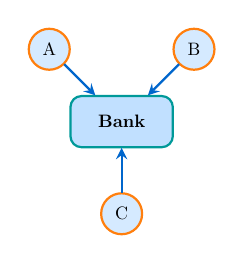
\begin{tikzpicture}[scale=0.65, transform shape]
% Central ledger
\node (bank) [blockchain, minimum width=2cm] {\textbf{Bank}};
\node (alice) [transaction, above left of=bank, node distance=2cm] {A};
\node (bob) [transaction, above right of=bank, node distance=2cm] {B};
\node (carol) [transaction, below of=bank, node distance=1.8cm] {C};

\draw[arrow] (alice) -- (bank);
\draw[arrow] (bob) -- (bank);
\draw[arrow] (carol) -- (bank);
\end{tikzpicture}
\end{center}
\begin{itemize}\compactlist
\item Identity verified
\item Balances in database
\item Transfers update records
\item \textbf{Example:} Bank app showing your balance
\end{itemize}
\end{block}
\end{column}
\begin{column}{0.48\textwidth}
\begin{block}{Token-Based (Bearer)}
\begin{center}
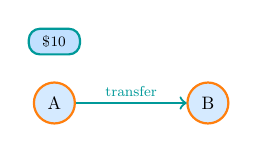
\begin{tikzpicture}[scale=0.65, transform shape]
% Direct transfer
\node (alice) [transaction] {A};
\node (bob) [transaction, right of=alice, node distance=3cm] {B};
\node (token) [blockchain, above of=alice, node distance=1.2cm, minimum width=1cm, minimum height=0.5cm] {\footnotesize \$10};

\draw[->, thick, dfteal] (alice) -- node[above] {\footnotesize transfer} (bob);
\end{tikzpicture}
\end{center}
\begin{itemize}\compactlist
\item Possession = ownership
\item No identity needed
\item Physical handoff
\item \textbf{Example:} Cash in your wallet
\end{itemize}
\end{block}
\end{column}
\end{columns}

\vspace{3mm}
\textbf{Visual comparison:} Checking your bank app balance (account-based) vs. counting cash in your wallet (token-based)

\vspace{2mm}
\begin{alertblock}{The Digital Dilemma}
Physical tokens can be handed over. Digital files can be \textbf{copied}. How do you hand over a digital token without copying it?
\end{alertblock}
\end{frame}

% =============================================================================
% Frame 12: Why Physical Money Works
% =============================================================================
\begin{frame}{Why Physical Money Works}
\begin{center}
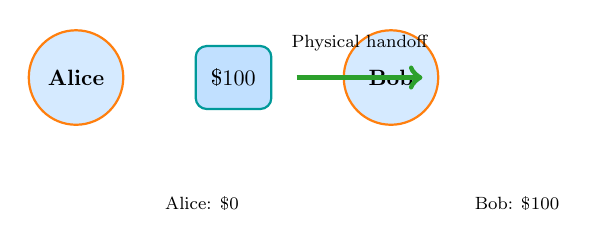
\begin{tikzpicture}[scale=0.8, transform shape]
% Physical transfer
\node (alice) [transaction, minimum size=1.5cm] {\textbf{Alice}};
\node (bill) [blockchain, right of=alice, node distance=2.5cm, minimum width=1.2cm] {\$100};
\node (bob) [transaction, right of=bill, node distance=2.5cm, minimum size=1.5cm] {\textbf{Bob}};

% Arrow showing transfer
\draw[->, thick, dfgreen, line width=2pt] (3.5,0) -- (5.5,0);
\node[above] at (4.5,0.3) {\footnotesize Physical handoff};

% After transfer
\node at (2,-2) {\footnotesize Alice: \$0};
\node at (7,-2) {\footnotesize Bob: \$100};
\end{tikzpicture}
\end{center}

\vspace{3mm}
\textbf{Physics enforces scarcity:}
\begin{itemize}
\item A physical object can only be in \textbf{one place} at a time
\item Giving it away means you \textbf{no longer have it}
\item No need to check a database---possession is proof
\end{itemize}

\begin{block}{Key Insight}
Physical money is \textbf{self-proving}. The laws of physics prevent double-spending automatically.
\end{block}
\end{frame}

% =============================================================================
% Frame 13: The Problem with Digital Files
% =============================================================================
\begin{frame}{The Problem with Digital Files}
\begin{center}
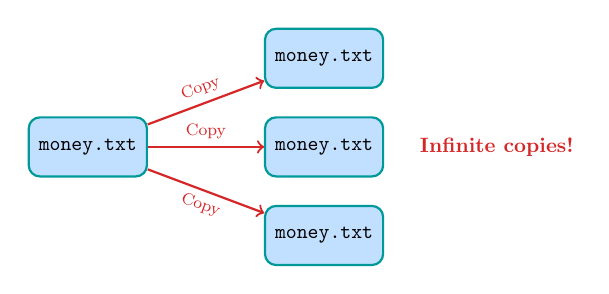
\begin{tikzpicture}[scale=0.75, transform shape]
% Original file
\node (original) [blockchain, minimum width=2cm] at (0,0) {\texttt{money.txt}};

% Copies
\node (copy1) [blockchain, minimum width=2cm] at (4,1.5) {\texttt{money.txt}};
\node (copy2) [blockchain, minimum width=2cm] at (4,0) {\texttt{money.txt}};
\node (copy3) [blockchain, minimum width=2cm] at (4,-1.5) {\texttt{money.txt}};

% Arrows
\draw[->, thick, dfred] (original) -- node[above, sloped] {\footnotesize Copy} (copy1);
\draw[->, thick, dfred] (original) -- node[above] {\footnotesize Copy} (copy2);
\draw[->, thick, dfred] (original) -- node[below, sloped] {\footnotesize Copy} (copy3);

% Label
\node[right] at (5.5,0) {\textcolor{dfred}{\textbf{Infinite copies!}}};
\end{tikzpicture}
\end{center}

\vspace{3mm}
\textbf{Digital information is fundamentally different:}
\begin{itemize}
\item \textbf{Perfect copies} cost nothing to make
\item \textbf{No scarcity}---bits can be duplicated infinitely
\item \textbf{No physics} to enforce ``giving it away''
\end{itemize}

\begin{alertblock}{The Digital Money Problem}
If money is just a file, what stops someone from copying it and spending it twice?
\end{alertblock}
\end{frame}

% =============================================================================
% Frame 14: The Double-Spending Problem
% =============================================================================
\begin{frame}{The Double-Spending Problem}
\begin{center}
\textbf{\Large The Fundamental Challenge of Digital Money}
\end{center}

\begin{columns}[T]
\begin{column}{0.55\textwidth}
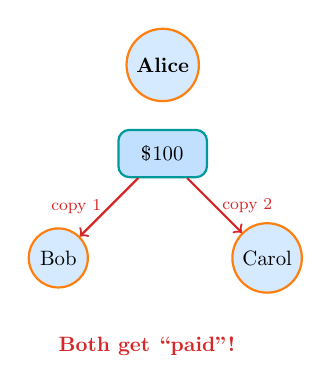
\begin{tikzpicture}[scale=0.75, transform shape, node distance=2cm]
% Alice with digital coin
\node (alice) [transaction, minimum size=1.2cm] {\textbf{Alice}};
\node (coin) [blockchain, below of=alice, minimum width=1.5cm, minimum height=0.8cm, node distance=1.5cm] {\$100};
\node (bob) [transaction, below left of=coin, minimum size=1cm, node distance=2.5cm] {Bob};
\node (carol) [transaction, below right of=coin, minimum size=1cm, node distance=2.5cm] {Carol};

% Arrows showing double spend
\draw[->, thick, dfred] (coin) -- node[left, font=\footnotesize] {copy 1} (bob);
\draw[->, thick, dfred] (coin) -- node[right, font=\footnotesize] {copy 2} (carol);

% Warning
\node[below of=bob, node distance=1.5cm, xshift=1.5cm] {\textcolor{dfred}{\textbf{Both get ``paid''!}}};
\end{tikzpicture}
\end{column}
\begin{column}{0.42\textwidth}
\textbf{Why is this hard?}
\begin{itemize}
\item Digital = perfectly copyable
\item No physical scarcity
\item Can't ``hand over'' a file
\item Need to prevent copies from both being valid
\end{itemize}

\vspace{2mm}
\textbf{How ledgers solve this:}\\
\footnotesize By keeping a single record everyone trusts

\vspace{2mm}
\textbf{Before 2008, only one solution existed:}\\
\textcolor{dfteal}{A trusted central authority}
\end{column}
\end{columns}
\end{frame}

% =============================================================================
% Frame 15: Double-Spending: A Concrete Example
% =============================================================================
\begin{frame}{Double-Spending: A Concrete Example}
\begin{center}
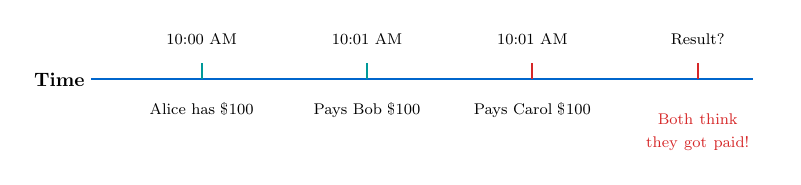
\begin{tikzpicture}[scale=0.7, transform shape]
% Timeline
\draw[thick, dfblue] (0,0) -- (12,0);
\node[left] at (0,0) {\textbf{Time}};

% Events
\node[above] at (2,0.5) {\footnotesize 10:00 AM};
\node[below] at (2,-0.3) {\footnotesize Alice has \$100};
\draw[thick, dfteal] (2,0) -- (2,0.3);

\node[above] at (5,0.5) {\footnotesize 10:01 AM};
\node[below] at (5,-0.3) {\footnotesize Pays Bob \$100};
\draw[thick, dfteal] (5,0) -- (5,0.3);

\node[above] at (8,0.5) {\footnotesize 10:01 AM};
\node[below] at (8,-0.3) {\footnotesize Pays Carol \$100};
\draw[thick, dfred] (8,0) -- (8,0.3);

\node[above] at (11,0.5) {\footnotesize Result?};
\node[below, text width=2.5cm, align=center] at (11,-0.5) {\textcolor{dfred}{\footnotesize Both think they got paid!}};
\draw[thick, dfred] (11,0) -- (11,0.3);
\end{tikzpicture}
\end{center}

\vspace{5mm}
\textbf{Without a central authority:}
\begin{itemize}
\item Bob checks his copy of the ledger: ``Alice paid me \$100'' \checkmark
\item Carol checks her copy: ``Alice paid me \$100'' \checkmark
\item Neither knows about the other transaction!
\end{itemize}

\begin{block}{The Core Question}
How do Bob and Carol \textbf{agree} on which transaction is valid?
\end{block}
\end{frame}

% =============================================================================
% Frame 16: The Traditional Solution: Trusted Third Parties
% =============================================================================
\begin{frame}{The Traditional Solution: Trusted Third Parties}
\begin{center}
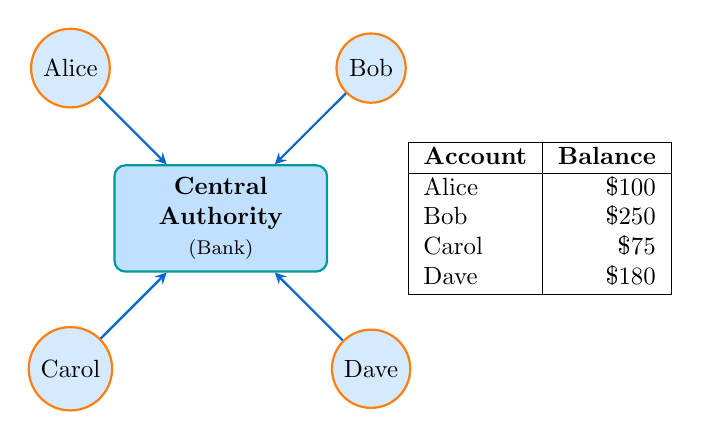
\begin{tikzpicture}[scale=0.9, transform shape]
% Central authority
\node (bank) [blockchain, minimum width=3cm, minimum height=1.5cm] {
\begin{tabular}{c}
\textbf{Central}\\
\textbf{Authority}\\
\footnotesize (Bank)
\end{tabular}
};

% Users around
\node (alice) [transaction, above left of=bank, node distance=3cm] {Alice};
\node (bob) [transaction, above right of=bank, node distance=3cm] {Bob};
\node (carol) [transaction, below left of=bank, node distance=3cm] {Carol};
\node (dave) [transaction, below right of=bank, node distance=3cm] {Dave};

% Connections
\draw[arrow] (alice) -- (bank);
\draw[arrow] (bob) -- (bank);
\draw[arrow] (carol) -- (bank);
\draw[arrow] (dave) -- (bank);

% Ledger
\node[right of=bank, node distance=4.5cm] {
\begin{tabular}{|l|r|}
\hline
\textbf{Account} & \textbf{Balance} \\
\hline
Alice & \$100 \\
Bob & \$250 \\
Carol & \$75 \\
Dave & \$180 \\
\hline
\end{tabular}
};
\end{tikzpicture}
\end{center}

\textbf{How it prevents double-spending:}
\begin{enumerate}
\item Alice requests: ``Send \$100 to Bob''
\item Bank checks: Does Alice have \$100?
\item Bank updates: Alice $-$\$100, Bob $+$\$100
\item Transaction complete---Alice can't spend it again
\end{enumerate}
\end{frame}

% =============================================================================
% Frame 17: How Banks Validate Transactions
% =============================================================================
\begin{frame}{How Banks Validate Transactions}
\begin{center}
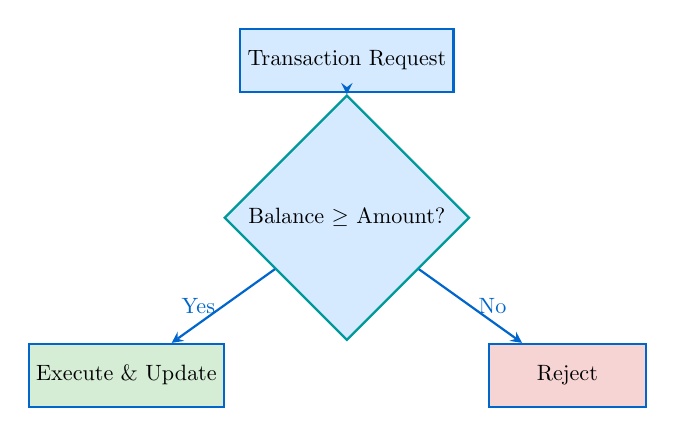
\begin{tikzpicture}[scale=0.8, transform shape]
% Flow chart
\node[process, minimum width=2.5cm] (request) at (0,3) {Transaction Request};
\node[decision, minimum width=2cm] (check) at (0,0.5) {Balance $\geq$ Amount?};
\node[process, fill=dfgreen!20, minimum width=2.5cm] (approve) at (-3.5,-2) {Execute \& Update};
\node[process, fill=dfred!20, minimum width=2.5cm] (reject) at (3.5,-2) {Reject};

\draw[arrow] (request) -- (check);
\draw[arrow] (check) -- node[left] {Yes} (approve);
\draw[arrow] (check) -- node[right] {No} (reject);
\end{tikzpicture}
\end{center}

\textbf{Key Properties:}
\begin{itemize}
\item \textbf{Sequential processing:} One transaction at a time
\item \textbf{Atomic execution:} All-or-nothing (no partial transfers)
\item \textbf{Single source of truth:} Only the bank's ledger matters
\end{itemize}
\end{frame}

% =============================================================================
% Frame 18: The Cost of Trust - What We Gain
% =============================================================================
\begin{frame}{The Cost of Trust: What We Gain}
\begin{columns}[T]
\begin{column}{0.48\textwidth}
\textbf{Benefits of Trusted Intermediaries:}

\vspace{3mm}
\begin{itemize}
\item[\textcolor{dfgreen}{\checkmark}] \textbf{Double-spending prevented}\\
\footnotesize Central validation ensures no duplicate spending

\item[\textcolor{dfgreen}{\checkmark}] \textbf{Transaction records}\\
\footnotesize Complete audit trail maintained

\item[\textcolor{dfgreen}{\checkmark}] \textbf{Dispute resolution}\\
\footnotesize Authority can mediate conflicts

\item[\textcolor{dfgreen}{\checkmark}] \textbf{Reversibility}\\
\footnotesize Chargebacks possible for fraud
\end{itemize}
\end{column}
\begin{column}{0.48\textwidth}
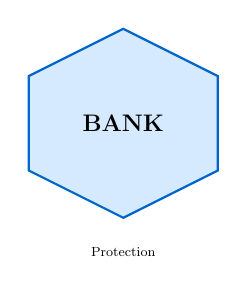
\begin{tikzpicture}[scale=0.6, transform shape]
% Shield icon
\draw[thick, dfblue, fill=dflightblue4] (2,0) -- (0,1) -- (0,3) -- (2,4) -- (4,3) -- (4,1) -- cycle;
\node at (2,2) {\Large \textbf{BANK}};
\node[below] at (2,-0.5) {\footnotesize Protection};
\end{tikzpicture}

\vspace{5mm}
\begin{block}{The Value Proposition}
``Trust us, and we'll protect your money.''
\end{block}
\end{column}
\end{columns}
\end{frame}

% =============================================================================
% Frame 19: The Cost of Trust - What We Lose
% =============================================================================
\begin{frame}{The Cost of Trust: What We Lose}
\begin{columns}[T]
\begin{column}{0.48\textwidth}
\textbf{Costs of Centralization:}

\vspace{3mm}
\begin{itemize}
\item[\textcolor{dfred}{$\times$}] \textbf{Privacy}\\
\footnotesize Bank sees all transactions

\item[\textcolor{dfred}{$\times$}] \textbf{Autonomy}\\
\footnotesize Bank can freeze accounts

\item[\textcolor{dfred}{$\times$}] \textbf{Inclusion}\\
\footnotesize Need bank approval to participate

\item[\textcolor{dfred}{$\times$}] \textbf{Speed}\\
\footnotesize Bank's hours and processes

\item[\textcolor{dfred}{$\times$}] \textbf{Cost}\\
\footnotesize Fees of 1--5\% or more
\end{itemize}
\end{column}
\begin{column}{0.48\textwidth}
\begin{alertblock}{The Trust Assumption}
We must trust that the central authority:
\begin{itemize}\compactlist
\item Won't steal our money
\item Won't censor transactions
\item Won't fail or get hacked
\item Will always be available
\item Will treat everyone fairly
\end{itemize}
\end{alertblock}

\vspace{2mm}
\textbf{2008 Financial Crisis:}\\
\footnotesize Many questioned whether this trust was warranted.
\end{column}
\end{columns}
\end{frame}

% =============================================================================
% Frame 20: Counterparty Risk
% =============================================================================
\begin{frame}{Counterparty Risk: When Trust Fails}
\begin{columns}[T]
\begin{column}{0.55\textwidth}
\textbf{What is Counterparty Risk?}

The risk that the other party (bank) might fail to fulfill its obligations.

\vspace{3mm}
\textbf{Examples:}
\begin{itemize}
\item Bank becomes insolvent
\item Bank run depletes reserves
\item Government seizes assets
\item Cyberattack compromises systems
\end{itemize}

\vspace{2mm}
\textbf{2008 Financial Crisis:}
\footnotesize In 2008, banks didn't trust each other's IOUs---the interbank lending system froze
\end{column}
\begin{column}{0.42\textwidth}
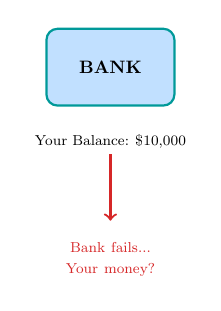
\begin{tikzpicture}[scale=0.65, transform shape]
% Bank failure visualization
\node[blockchain, minimum width=2.5cm, minimum height=1.5cm] (bank) at (0,2) {\textbf{BANK}};
\node[below] at (0,0.8) {\footnotesize Your Balance: \$10,000};

\draw[thick, dfred, ->] (0,0.3) -- (0,-1);
\node[below, text width=3cm, align=center] at (0,-1.3) {\textcolor{dfred}{\footnotesize Bank fails...\\Your money?}};
\end{tikzpicture}
\end{column}
\end{columns}

\vspace{3mm}
\begin{block}{Fractional Reserve Banking}
\textbf{Simple example:} You deposit \$100. The bank keeps \$10 and lends \$90 to someone else. Your account still shows \$100.

\vspace{2mm}
If everyone withdraws at once, the bank cannot pay. This is called a \textbf{bank run}.
\end{block}
\end{frame}

% =============================================================================
% Frame 21: Censorship and Exclusion
% =============================================================================
\begin{frame}{Censorship and Exclusion}
\begin{columns}[T]
\begin{column}{0.55\textwidth}
\textbf{Censorship Risk:}
\begin{itemize}
\item Accounts can be frozen
\item Transactions can be blocked
\item Access can be revoked
\item No permission = no participation
\end{itemize}

\vspace{2mm}
\textbf{What happens when the TTP fails?}
\footnotesize Example: What if PayPal freezes your account?

\vspace{3mm}
\textbf{Financial Exclusion:}
\begin{itemize}
\item \textbf{1.4 billion adults} worldwide lack bank access
\item Requirements: ID, minimum balance, credit check
\item Geographic limitations
\item 3--5 day international transfers
\end{itemize}
\end{column}
\begin{column}{0.42\textwidth}
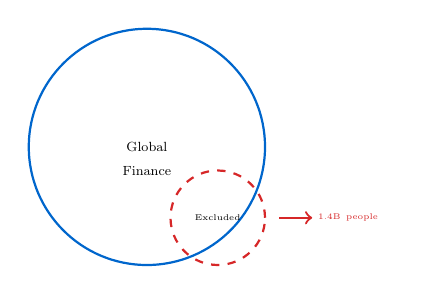
\begin{tikzpicture}[scale=0.6, transform shape]
% World with excluded regions
\draw[thick, dfblue] (0,0) circle (2.5cm);
\node at (0,0) {\footnotesize Global};
\node at (0,-0.5) {\footnotesize Finance};

% Excluded
\draw[thick, dfred, dashed] (1.5,-1.5) circle (1cm);
\node at (1.5,-1.5) {\tiny Excluded};

% Arrow
\draw[->, thick, dfred] (2.8,-1.5) -- (3.5,-1.5);
\node[right, text width=1.5cm] at (3.5,-1.5) {\tiny \textcolor{dfred}{1.4B people}};
\end{tikzpicture}

\vspace{3mm}
\begin{alertblock}{Key Question}
Should access to money require permission?
\end{alertblock}
\end{column}
\end{columns}
\end{frame}

% =============================================================================
% Frame 22: The Byzantine Generals Problem
% =============================================================================
\begin{frame}{The Coordination Problem: Byzantine Generals}
\begin{columns}[T]
\begin{column}{0.55\textwidth}
\textbf{The Thought Experiment:}

Several generals surround an enemy city. They must coordinate to attack together or retreat together. But:
\begin{itemize}
\item Generals can only communicate via messengers
\item Some messengers might be \textbf{traitors}
\item Some generals might be \textbf{traitors}
\end{itemize}

\vspace{3mm}
\textbf{The Challenge:}\\
How do loyal generals agree on a plan when they can't trust all messages or all participants?
\end{column}
\begin{column}{0.42\textwidth}
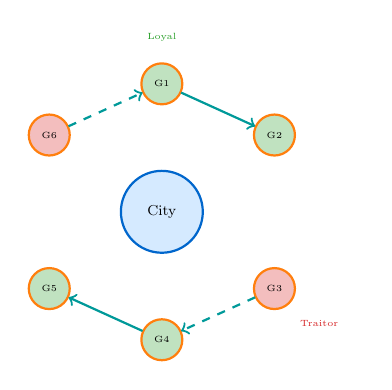
\begin{tikzpicture}[scale=0.65, transform shape]
% City in center
\draw[thick, dfblue, fill=dflightblue4] (0,0) circle (0.8cm);
\node at (0,0) {\footnotesize City};

% Generals around city
\node[transaction, minimum size=0.8cm, fill=dfgreen!30] (g1) at (0,2.5) {\tiny G1};
\node[transaction, minimum size=0.8cm, fill=dfgreen!30] (g2) at (2.2,1.5) {\tiny G2};
\node[transaction, minimum size=0.8cm, fill=dfred!30] (g3) at (2.2,-1.5) {\tiny G3};
\node[transaction, minimum size=0.8cm, fill=dfgreen!30] (g4) at (0,-2.5) {\tiny G4};
\node[transaction, minimum size=0.8cm, fill=dfgreen!30] (g5) at (-2.2,-1.5) {\tiny G5};
\node[transaction, minimum size=0.8cm, fill=dfred!30] (g6) at (-2.2,1.5) {\tiny G6};

% Message arrows (some solid, some dashed for unreliable)
\draw[->, dfteal, thick] (g1) -- (g2);
\draw[->, dfteal, thick, dashed] (g3) -- (g4);
\draw[->, dfteal, thick] (g4) -- (g5);
\draw[->, dfteal, thick, dashed] (g6) -- (g1);

% Labels
\node[above, text width=1.5cm, align=center] at (0,3.2) {\tiny \textcolor{dfgreen}{Loyal}};
\node[below right, text width=1.5cm, align=center] at (2.2,-2) {\tiny \textcolor{dfred}{Traitor}};
\end{tikzpicture}

\vspace{2mm}
\begin{alertblock}{Key Insight}
This is the fundamental problem of \textbf{consensus without trust}.
\end{alertblock}
\end{column}
\end{columns}
\end{frame}

% =============================================================================
% Frame 23: Byzantine Generals and Money
% =============================================================================
\begin{frame}{From Generals to Money: The Same Problem}
\begin{center}
\textbf{\Large ``How do strangers agree on who owns what without trusting each other?''}
\end{center}

\vspace{5mm}
\begin{columns}[T]
\begin{column}{0.48\textwidth}
\textbf{The Parallel:}
\begin{itemize}
\item \textbf{Generals} = Network participants
\item \textbf{City attack plan} = Transaction history
\item \textbf{Traitors} = Malicious actors trying to double-spend
\item \textbf{Messages} = Transaction broadcasts
\end{itemize}
\end{column}
\begin{column}{0.48\textwidth}
\textbf{The Challenge:}
\begin{itemize}
\item Alice sends conflicting messages: ``I paid Bob'' and ``I paid Carol''
\item Bob and Carol each see one message
\item Who should they believe?
\item How do they agree on what really happened?
\end{itemize}
\end{column}
\end{columns}

\vspace{5mm}
\begin{block}{Why This Matters}
Before Bitcoin (2008), there was \textbf{no known solution} to the Byzantine Generals Problem for large, open networks. This is why digital money required trusted banks. Blockchain changed everything.
\end{block}
\end{frame}

% =============================================================================
% Frame 24: The Quest for Digital Cash
% =============================================================================
\begin{frame}{The Quest for Digital Cash}
\begin{center}
\textbf{\Large Can we have the benefits of cash in digital form?}
\end{center}

\vspace{3mm}
\begin{columns}[T]
\begin{column}{0.48\textwidth}
\textbf{Cash Properties:}
\begin{itemize}
\item[\textcolor{dfgreen}{\checkmark}] No permission needed
\item[\textcolor{dfgreen}{\checkmark}] Instant settlement
\item[\textcolor{dfgreen}{\checkmark}] Privacy (no tracking)
\item[\textcolor{dfgreen}{\checkmark}] No counterparty risk
\item[\textcolor{dfgreen}{\checkmark}] No censorship
\end{itemize}
\end{column}
\begin{column}{0.48\textwidth}
\textbf{Digital Requirements:}
\begin{itemize}
\item Works over the internet
\item Globally accessible
\item Divisible to small amounts
\item Programmable
\item Secure against copying
\end{itemize}
\end{column}
\end{columns}

\vspace{5mm}
\begin{block}{The Challenge}
How do you prevent double-spending digitally \textbf{without} a central authority?
\end{block}
\end{frame}

% =============================================================================
% Frame 25: Early Attempts at Digital Cash
% =============================================================================
\begin{frame}{Early Attempts at Digital Cash}
\begin{center}
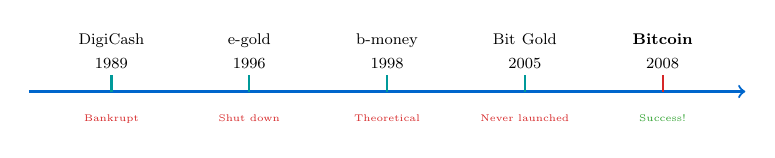
\begin{tikzpicture}[scale=0.7, transform shape]
% Timeline
\draw[thick, dfblue, ->] (0,0) -- (13,0);

% Projects
\node[above, text width=1.8cm, align=center] at (1.5,0.3) {\footnotesize DigiCash\\1989};
\draw[thick, dfteal] (1.5,0) -- (1.5,0.3);

\node[above, text width=1.8cm, align=center] at (4,0.3) {\footnotesize e-gold\\1996};
\draw[thick, dfteal] (4,0) -- (4,0.3);

\node[above, text width=1.8cm, align=center] at (6.5,0.3) {\footnotesize b-money\\1998};
\draw[thick, dfteal] (6.5,0) -- (6.5,0.3);

\node[above, text width=1.8cm, align=center] at (9,0.3) {\footnotesize Bit Gold\\2005};
\draw[thick, dfteal] (9,0) -- (9,0.3);

\node[above, text width=1.8cm, align=center] at (11.5,0.3) {\footnotesize \textbf{Bitcoin}\\2008};
\draw[thick, dfred] (11.5,0) -- (11.5,0.3);

% Failures
\node[below] at (1.5,-0.3) {\textcolor{dfred}{\tiny Bankrupt}};
\node[below] at (4,-0.3) {\textcolor{dfred}{\tiny Shut down}};
\node[below] at (6.5,-0.3) {\textcolor{dfred}{\tiny Theoretical}};
\node[below] at (9,-0.3) {\textcolor{dfred}{\tiny Never launched}};
\node[below] at (11.5,-0.3) {\textcolor{dfgreen}{\tiny Success!}};
\end{tikzpicture}
\end{center}

\vspace{3mm}
\textbf{Why did earlier attempts fail?}
\begin{itemize}
\item Still relied on central parties (company, servers)
\item Legal/regulatory shutdown
\item No solution to Byzantine consensus
\end{itemize}
\end{frame}

% =============================================================================
% Frame 26: The Bitcoin Breakthrough (Preview)
% =============================================================================
\begin{frame}{The Bitcoin Breakthrough (Preview)}
\begin{center}
\textbf{\Large What if we could prevent double-spending \textit{without} a central authority?}
\end{center}

\vspace{3mm}
\begin{columns}[T]
\begin{column}{0.48\textwidth}
\textbf{Satoshi Nakamoto's insight:}
\begin{enumerate}
\item Replicate the ledger everywhere
\item Use cryptography to verify
\item Use economic incentives to secure
\item Achieve consensus without trust
\end{enumerate}
\end{column}
\begin{column}{0.48\textwidth}
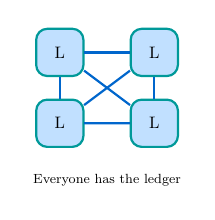
\begin{tikzpicture}[scale=0.6, transform shape]
% Distributed network
\node (n1) [blockchain, minimum width=1cm] {L};
\node (n2) [blockchain, right of=n1, node distance=2cm, minimum width=1cm] {L};
\node (n3) [blockchain, below of=n1, node distance=1.5cm, minimum width=1cm] {L};
\node (n4) [blockchain, below of=n2, node distance=1.5cm, minimum width=1cm] {L};

\draw[thick, dfblue] (n1) -- (n2);
\draw[thick, dfblue] (n1) -- (n3);
\draw[thick, dfblue] (n1) -- (n4);
\draw[thick, dfblue] (n2) -- (n3);
\draw[thick, dfblue] (n2) -- (n4);
\draw[thick, dfblue] (n3) -- (n4);

\node[below of=n3, node distance=1.2cm, xshift=1cm] {\footnotesize Everyone has the ledger};
\end{tikzpicture}
\end{column}
\end{columns}

\vspace{5mm}
\begin{block}{We'll Explore This in Topic 1.2}
For now, understand that \textbf{blockchain} is one answer to: ``How do we have digital money without trusting a single party?''
\end{block}
\end{frame}

% =============================================================================
% Frame 27: Hands-On Exercise I
% =============================================================================
\begin{frame}{Hands-On: Ledger Simulation}
\begin{center}
\textbf{\Large Let's See Double-Spending in Action}
\end{center}

\vspace{5mm}
\textbf{In the Colab notebook (NB01), we will:}
\begin{enumerate}
\item Build a simple ledger with account balances
\item Process valid transactions
\item Attempt a double-spend attack
\item See how a central authority prevents it
\item Discuss: What happens without the authority?
\end{enumerate}

\vspace{5mm}
\begin{block}{Access the Notebook}
\texttt{day\_01/notebooks/NB01\_ledger\_simulation.ipynb}

\vspace{2mm}
\footnotesize Or scan QR code / click link provided
\end{block}

\bottomnote{Time: 15-20 minutes for guided exploration}
\end{frame}

% =============================================================================
% Frame 28: Hands-On Exercise II - What You'll Learn
% =============================================================================
\begin{frame}{Notebook Objectives}
\begin{columns}[T]
\begin{column}{0.48\textwidth}
\textbf{Part 1: Build a Ledger}
\begin{itemize}
\item Create accounts with balances
\item Implement transfer function
\item Add balance validation
\end{itemize}

\vspace{3mm}
\textbf{Part 2: Test Double-Spending}
\begin{itemize}
\item Create a malicious transaction
\item Observe the attack
\item Understand why it works/fails
\end{itemize}
\end{column}
\begin{column}{0.48\textwidth}
\textbf{Part 3: Explore Trade-offs}
\begin{itemize}
\item Centralized vs. no central authority
\item Speed vs. security
\item Privacy vs. auditability
\end{itemize}

\vspace{3mm}
\begin{alertblock}{Key Takeaway}
Understanding \textit{why} the problem is hard helps you appreciate blockchain's solution.
\end{alertblock}
\end{column}
\end{columns}
\end{frame}

% =============================================================================
% Frame 29: Discussion: Money in the Digital Age
% =============================================================================
\begin{frame}{Discussion: Money in the Digital Age}
\begin{columns}[T]
\begin{column}{0.48\textwidth}
\textbf{Questions to Consider:}
\begin{enumerate}
\item Is Bitcoin ``real money''? Why or why not?
\item What makes you trust your bank?
\item If you could design money from scratch, what would it look like?
\item Is privacy a feature or a bug?
\end{enumerate}
\end{column}
\begin{column}{0.48\textwidth}
\textbf{Key Takeaways:}
\begin{itemize}
\item Money = trust infrastructure
\item Digital money needs double-spend protection
\item Central authorities work but have costs
\item Blockchain offers an alternative
\end{itemize}
\end{column}
\end{columns}

\vspace{5mm}
\begin{alertblock}{The Central Question of This Course}
How should we build the trust infrastructure for a digital economy?
\end{alertblock}
\end{frame}

% =============================================================================
% Frame 30: Application: Comparing Money Systems
% =============================================================================
\begin{frame}{Application: Comparing Money Systems}
\begin{center}
\footnotesize
\begin{tabular}{lccccc}
\toprule
\textbf{Property} & \textbf{Cash} & \textbf{Bank} & \textbf{PayPal} & \textbf{Bitcoin} & \textbf{Stablecoin} \\
\midrule
Speed & Fast & Slow & Medium & Slow & Fast \\
Privacy & High & Low & Low & Medium & Medium \\
Reversibility & No & Yes & Yes & No & Varies \\
Permission & No & Yes & Yes & No & No \\
Censorship & Hard & Easy & Easy & Hard & Medium \\
Global & No & Limited & Yes & Yes & Yes \\
\bottomrule
\end{tabular}
\end{center}

\vspace{3mm}
\textbf{Key Insight:} No single system is ``best.'' Each optimizes for different properties.

\begin{block}{Design Trade-offs}
Every money system makes choices about what to prioritize. Understanding these trade-offs is essential for evaluating new financial technologies.
\end{block}
\end{frame}

% =============================================================================
% Frame 31: Real-World Applications
% =============================================================================
\begin{frame}{Real-World Applications}
\begin{columns}[T]
\begin{column}{0.48\textwidth}
\textbf{Where This Matters:}

\vspace{2mm}
\textbf{Remittances}
\begin{itemize}\compactlist
\item \$700B+ sent globally per year
\item Fees average 6--7\%
\item 3--5 days for settlement
\end{itemize}

\vspace{2mm}
\textbf{Financial Inclusion}
\begin{itemize}\compactlist
\item 1.4B unbanked adults
\item Mobile phones more common than banks
\item Crypto as access point
\end{itemize}
\end{column}
\begin{column}{0.48\textwidth}
\textbf{Cross-Border Commerce}
\begin{itemize}\compactlist
\item Currency conversion costs
\item Settlement delays
\item Regulatory friction
\end{itemize}

\vspace{2mm}
\textbf{Economic Instability}
\begin{itemize}\compactlist
\item Hyperinflation (Venezuela, Zimbabwe)
\item Capital controls
\item Currency devaluation
\end{itemize}

\vspace{3mm}
\begin{block}{Implication}
Understanding money's foundations helps evaluate proposed solutions.
\end{block}
\end{column}
\end{columns}
\end{frame}

% =============================================================================
% Frame 32: The Future of Money
% =============================================================================
\begin{frame}{The Future of Money}
\begin{center}
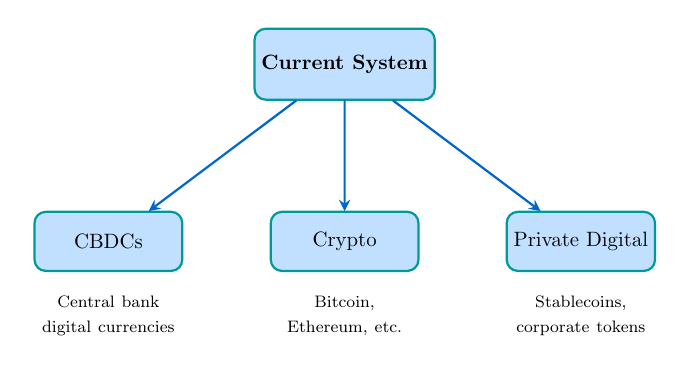
\begin{tikzpicture}[scale=0.75, transform shape]
% Three paths
\node[blockchain, minimum width=3cm, minimum height=1.2cm] (current) at (0,3) {\textbf{Current System}};

\node[blockchain, minimum width=2.5cm] (cbdc) at (-4,0) {CBDCs};
\node[blockchain, minimum width=2.5cm] (crypto) at (0,0) {Crypto};
\node[blockchain, minimum width=2.5cm] (private) at (4,0) {Private Digital};

\draw[arrow] (current) -- (cbdc);
\draw[arrow] (current) -- (crypto);
\draw[arrow] (current) -- (private);

% Labels
\node[below, text width=2.5cm, align=center] at (-4,-0.8) {\footnotesize Central bank digital currencies};
\node[below, text width=2.5cm, align=center] at (0,-0.8) {\footnotesize Bitcoin, Ethereum, etc.};
\node[below, text width=2.5cm, align=center] at (4,-0.8) {\footnotesize Stablecoins, corporate tokens};
\end{tikzpicture}
\end{center}

\vspace{3mm}
\textbf{Emerging Questions:}
\begin{itemize}
\item Who should control digital money?
\item How do we balance privacy and regulation?
\item Can different systems coexist?
\end{itemize}
\end{frame}

% =============================================================================
% Frame 33: Executive Summary
% =============================================================================
\begin{frame}{Executive Summary}
\begin{center}
\textbf{\Large Key Takeaways from Topic 1.1}
\end{center}

\vspace{3mm}
\begin{enumerate}
\item \textbf{Money is information, not objects}\\
\footnotesize Ledgers and trust predate physical currency

\item \textbf{The double-spending problem is fundamental}\\
\footnotesize Digital files can be copied; money cannot be

\item \textbf{Traditional solution: trusted intermediaries}\\
\footnotesize Banks prevent double-spending but introduce costs

\item \textbf{Costs include:} fees, delays, exclusion, censorship, counterparty risk

\item \textbf{Blockchain proposes an alternative}\\
\footnotesize Decentralized consensus without central trust
\end{enumerate}

\vspace{3mm}
\begin{block}{The Big Idea}
Understanding \textit{why} digital money is hard helps you appreciate \textit{how} blockchain solves it.
\end{block}
\end{frame}

% =============================================================================
% Frame 34: Concept Map
% =============================================================================
\begin{frame}{Concept Map: Money and Trust}
\begin{center}
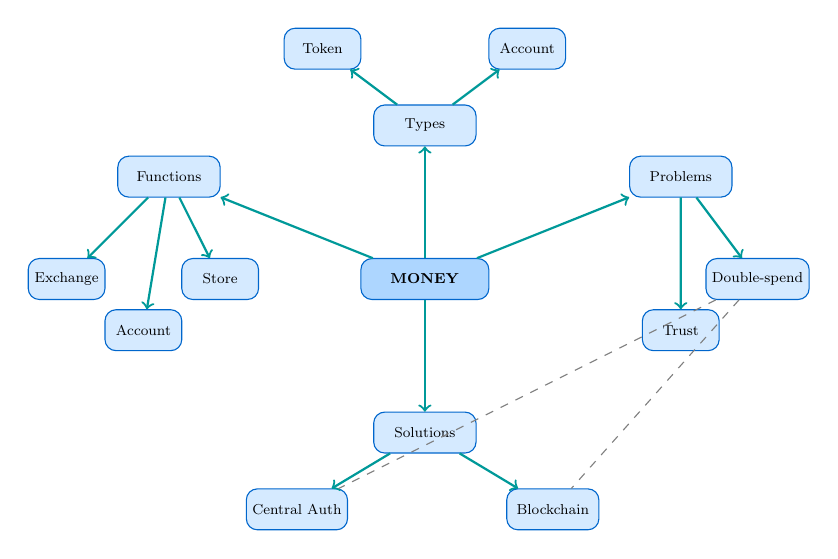
\begin{tikzpicture}[scale=0.65, transform shape,
    concept/.style={rectangle, rounded corners, draw=dfblue, fill=dflightblue4, minimum width=2cm, minimum height=0.8cm, font=\footnotesize},
    relationship/.style={->, thick, dfteal}]

% Central concept
\node[concept, fill=dflightblue2, minimum width=2.5cm] (money) at (0,0) {\textbf{MONEY}};

% Main branches
\node[concept] (functions) at (-5,2) {Functions};
\node[concept] (types) at (0,3) {Types};
\node[concept] (problems) at (5,2) {Problems};
\node[concept] (solutions) at (0,-3) {Solutions};

% Functions
\node[concept, minimum width=1.5cm] (exchange) at (-7,0) {Exchange};
\node[concept, minimum width=1.5cm] (account) at (-5.5,-1) {Account};
\node[concept, minimum width=1.5cm] (store) at (-4,0) {Store};

% Types
\node[concept, minimum width=1.5cm] (token) at (-2,4.5) {Token};
\node[concept, minimum width=1.5cm] (acct) at (2,4.5) {Account};

% Problems
\node[concept, minimum width=1.8cm] (double) at (6.5,0) {Double-spend};
\node[concept, minimum width=1.5cm] (trust) at (5,-1) {Trust};

% Solutions
\node[concept, minimum width=1.8cm] (central) at (-2.5,-4.5) {Central Auth};
\node[concept, minimum width=1.8cm] (blockchain) at (2.5,-4.5) {Blockchain};

% Connections
\draw[relationship] (money) -- (functions);
\draw[relationship] (money) -- (types);
\draw[relationship] (money) -- (problems);
\draw[relationship] (money) -- (solutions);

\draw[relationship] (functions) -- (exchange);
\draw[relationship] (functions) -- (account);
\draw[relationship] (functions) -- (store);

\draw[relationship] (types) -- (token);
\draw[relationship] (types) -- (acct);

\draw[relationship] (problems) -- (double);
\draw[relationship] (problems) -- (trust);

\draw[relationship] (solutions) -- (central);
\draw[relationship] (solutions) -- (blockchain);

% Cross-connections
\draw[dashed, dfgray] (double) -- (central);
\draw[dashed, dfgray] (double) -- (blockchain);
\end{tikzpicture}
\end{center}
\end{frame}

% =============================================================================
% Frame 35: Key Terms & Definitions I
% =============================================================================
\begin{frame}{Key Terms \& Definitions (I)}
\begin{description}
\item[Money] A social technology that serves as medium of exchange, unit of account, and store of value---fundamentally based on trust.

\item[Ledger] A record of transactions showing who owes what to whom; humanity's oldest financial technology.

\item[Double-Spending] The fundamental challenge of digital money: spending the same digital value multiple times because files can be copied.

\item[Token-Based Money] Bearer instruments where possession equals ownership (e.g., cash, gold coins).

\item[Account-Based Money] Systems where identity is verified and balances are tracked in a central database (e.g., bank accounts).
\end{description}
\end{frame}

% =============================================================================
% Frame 36: Key Terms & Definitions II
% =============================================================================
\begin{frame}{Key Terms \& Definitions (II)}
\begin{description}
\item[Trusted Third Party] A central authority (like a bank) that validates transactions and maintains the authoritative ledger.

\item[Counterparty Risk] The risk that the other party (e.g., bank) might fail to fulfill its obligations.

\item[Fractional Reserve] Banking practice where banks keep only a fraction (e.g., 10\%) of deposits as reserves and lend the rest.

\item[Censorship Risk] The ability of authorities to freeze accounts, block transactions, or deny service.

\item[Atomic Execution] Transactions that complete fully or not at all---no partial states allowed.

\item[Single Source of Truth] One authoritative ledger that all parties must accept as correct.
\end{description}
\end{frame}

% =============================================================================
% Frame 37: Common Misconceptions
% =============================================================================
\begin{frame}{Common Misconceptions}
\begin{columns}[T]
\begin{column}{0.48\textwidth}
\textbf{\textcolor{dfred}{Misconception}}

\vspace{2mm}
``Money is backed by gold''

\vspace{5mm}
``Banks store your exact dollars''

\vspace{5mm}
``Digital = automatically better''

\vspace{5mm}
``Blockchain solves everything''
\end{column}
\begin{column}{0.48\textwidth}
\textbf{\textcolor{dfgreen}{Reality}}

\vspace{2mm}
Most currencies are fiat---backed by government promise and collective belief

\vspace{2mm}
Banks lend most deposits out (fractional reserve); your ``balance'' is an IOU

\vspace{2mm}
Digital creates the double-spend problem; requires new solutions

\vspace{2mm}
Blockchain is one solution with its own trade-offs; not universally superior
\end{column}
\end{columns}

\vspace{5mm}
\begin{alertblock}{Critical Thinking}
Always ask: What problem does this solve? What trade-offs does it introduce?
\end{alertblock}
\end{frame}

% =============================================================================
% Frame 38: Self-Assessment Question 1
% =============================================================================
\begin{frame}{Self-Assessment: Question 1}
\begin{block}{Question}
Which of the following is NOT one of the three fundamental functions of money?
\end{block}

\vspace{3mm}
\begin{enumerate}[A.]
\item Medium of exchange
\item Unit of account
\item Source of government revenue
\item Store of value
\end{enumerate}

\vspace{5mm}
\pause
\textbf{Answer: C}

\vspace{2mm}
\textbf{Explanation:} The three fundamental functions of money are: (1) medium of exchange (facilitating trade), (2) unit of account (measuring value), and (3) store of value (preserving purchasing power over time). While governments may collect taxes using money, generating revenue is not a core function of money itself.
\end{frame}

% =============================================================================
% Frame 39: Self-Assessment Questions 2-3
% =============================================================================
\begin{frame}{Self-Assessment: Questions 2-3}
\begin{block}{Question 2}
How do banks solve the double-spending problem in digital finance?
\end{block}
\textbf{Answer:} By maintaining a \textbf{centralized ledger} and validating every transaction against available balances before execution.

\vspace{5mm}
\begin{block}{Question 3}
What is fractional reserve banking?
\end{block}
\textbf{Answer:} A system where banks keep only a fraction (e.g., 10\%) of deposits as reserves and lend out the rest.

\vspace{3mm}
\textbf{Key Insight:} This enables economic growth but creates vulnerability during bank runs---not all depositors can withdraw simultaneously.
\end{frame}

% =============================================================================
% Frame 40: What's Next - Preview T1.2
% =============================================================================
\begin{frame}{What's Next: Topic 1.2}
\begin{center}
\textbf{\Large Preview: From Ledgers to Blockchains}
\end{center}

\vspace{5mm}
\textbf{In Topic 1.2, we'll explore:}
\begin{itemize}
\item How \textbf{cryptographic hashing} creates tamper-proof records
\item The structure of \textbf{blockchain} as a data structure
\item \textbf{Consensus mechanisms}---how strangers agree without trust
\item \textbf{Decentralization}---distributing the ledger to everyone
\end{itemize}

\vspace{5mm}
\begin{block}{Connection}
Topic 1.1 established the \textit{problem} (double-spending).\\
Topic 1.2 introduces the \textit{solution} (blockchain).
\end{block}

\vspace{3mm}
\textbf{Preparation:} Review the concepts of trust and ledgers from today's session.
\end{frame}

% =============================================================================
% Frame 41: Resources
% =============================================================================
\begin{frame}{Resources for Further Learning}
\textbf{Essential Reading:}
\begin{itemize}
\item Nakamoto, S. (2008). ``Bitcoin: A Peer-to-Peer Electronic Cash System''
\item Graeber, D. (2011). ``Debt: The First 5,000 Years'' (Ch. 1-3)
\end{itemize}

\vspace{3mm}
\textbf{Online Resources:}
\begin{itemize}
\item Course notebook: \texttt{NB01\_ledger\_simulation.ipynb}
\item World Bank Global Findex Database (unbanked statistics)
\item Bitcoin whitepaper: \url{bitcoin.org/bitcoin.pdf}
\end{itemize}

\vspace{3mm}
\textbf{Videos:}
\begin{itemize}
\item 3Blue1Brown: ``But how does bitcoin actually work?''
\item Antonopoulos: ``What is Money?'' (YouTube)
\end{itemize}

\vspace{3mm}
\begin{block}{Course Materials}
All slides and notebooks available on the course website.
\end{block}
\end{frame}

% =============================================================================
% Frame 42: Questions?
% =============================================================================
\begin{frame}{Questions?}
\begin{center}
\textbf{\LARGE Questions \& Discussion}

\vspace{10mm}
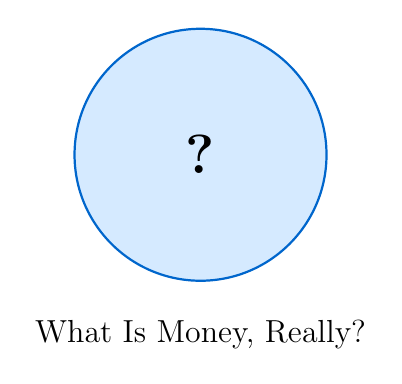
\begin{tikzpicture}[scale=0.8, transform shape]
% Question mark with money theme
\draw[thick, dfblue, fill=dflightblue4] (0,0) circle (2cm);
\node at (0,0) {\Huge \textbf{?}};
\node[below] at (0,-2.5) {\Large What Is Money, Really?};
\end{tikzpicture}

\vspace{10mm}
\textbf{Contact:} joerg.osterrieder@gmail.com

\vspace{3mm}
\textbf{Next Topic:} T1.2 --- From Ledgers to Blockchains
\end{center}
\end{frame}

\end{document}
